\section{Motivating Examples}
\label{sec:motivation}

As mentioned in Section 1, the programmer writes a Pig Latin program in an imperative style with high level declarative data transformation operations whose results can be assigned to an identifier which can be referred to later. The program is compiled to parallel map-reduce jobs through generation of logical and physical plan. The underlying compilation is hidden from the user and kep abstracted, away from the programmer's concern away. The programmer only needs to consider Pig Latin's simple high-level semantics.

The correctness of this compilation is of prime importance to state that the underlying map-reduce jobs will produce a correct output for any possible input data.

To clarify this process, consider the following example.

\subsection{Example 1:}
\label{subsec:example1}

The following example \cite{gates2009building} describes a simple Pig Latin program that takes two data sources file1 and file2 as input. performs a series of data transformations on them and finally stores the output.
\begin{lstlisting}
  A = LOAD 'file1' AS (x,y,z);
  B = LOAD 'file2' AS (t,u,v);
  C = FILTER A BY y>0;
  D = JOIN C BY x, B by u;
  E = GROUP D BY z;
  F = FOREACH E GENERATE group, COUNT(D);
  STORE F into 'output';
\end{lstlisting}

Here is an informal description of the meaning of this Pig Latin program:

\begin{itemize}
  \item Two files are loaded into variables \texttt{A} and \texttt{B}.
  \item \texttt{A} is filtered by a predicate the resulting data transformation operation is assigned to \texttt{C}.
	\item \texttt{D} represents the \texttt{JOIN} operation of \texttt{C} and \texttt{B}.
	\item The \texttt{GROUP BY} operation is assigned to the identifier \texttt{E}
	\item Finally, a \texttt{COUNT} aggregate function is applied to the relation \texttt{E} and the output is stored into \texttt{F}
	\item The output of computations of \texttt{f} are stored in a file \texttt{output}.
\end{itemize}

\begin{figure}
\begin{center}
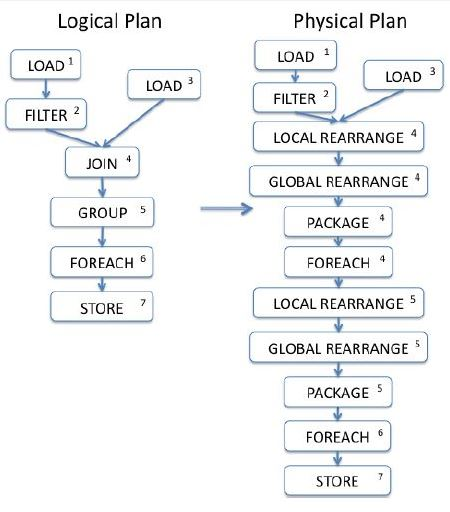
\includegraphics[scale=0.5]{Images/LogicalPhysicalPlan.JPG}
\end{center}
\caption{\textbf{Logical to Physical Plan} \cite{gates2009building}}
\end{figure}

Figure 1 shows how the program from this example is compiled to the logical plan and physical plan. Each data transformation operation in the original source program gets mapped one-to-one the nodes in logical plan. Each logical operator is annotated with a number corresponding to the operation by which it was defined in the program.

In this example, the logical plan is then translated into a physical plan where the \texttt{GROUP BY} operation is divided into a series of physical operators: \texttt{LOCAL REARRANGE}, \texttt{GLOBAL REARRANGE}, \texttt{PACKAGE}, and \texttt{FOREACH} operation. Corresponding logical and physical operators are annotated with the same id.
